%%%%%%%%%%%%%%%%%%%%%%%%%%%%%%%%%%%%%%%%%%%%%%
%                                            %
%   W Z O R Z E C   S P R A W O Z D A N I A  %
%                                            %
%%%%%%%%%%%%%%%%%%%%%%%%%%%%%%%%%%%%%%%%%%%%%%


\documentclass[12pt,a4paper,twoside]{article}

\usepackage{amsmath,amssymb}
\usepackage[utf8]{inputenc}                                      
\usepackage[OT4]{fontenc}      
%\usepackage[T1]{fontenc}                            
\usepackage[polish]{babel}                           
\selectlanguage{polish}
\usepackage{indentfirst} 
\usepackage[dvips]{graphicx}
\usepackage{tabularx}
\usepackage{color}
\usepackage{latexsym}
\usepackage{hyperref} 
\usepackage{fancyhdr}
\usepackage{listings}
\usepackage{booktabs}
\usepackage{ifpdf}
\usepackage{mathtext} % polskie znaki w trybie matematycznym
%\makeindex  % utworzenie skorowidza (w dokumencie pdf)
\usepackage{lmodern}
%\usepackage[osf]{libertine}
\usepackage{filecontents}
\usepackage{ifthen}
\usepackage{pdfpages}

\usepackage{tikz}
\usetikzlibrary{arrows}


\newcounter{nextYear}
\setcounter{nextYear}{\the\year}
\stepcounter{nextYear}

% rozszerzenie nieco strony
%\setlength{\topmargin}{-1cm} \setlength{\textheight}{24.5cm}
%\setlength{\textwidth}{17cm} \addtolength{\hoffset}{-1.5cm}
%\setlength{\parindent}{0.5cm} \setlength{\footskip}{2cm}
%\linespread{1.2} % odstep pomiedzy wierszami


%%%% ZYWA PAGINA %%%%%%%%%%%
\newcommand{\tl}[1]{\textbf{#1}} 
\pagestyle{fancy}
\renewcommand{\sectionmark}[1]{\markright{\thesection\ #1}}
\fancyhf{} % usuwanie bieżących ustawień
\fancyhead[LE,RO]{\small\bfseries\thepage}
\fancyhead[LO]{\small\bfseries\rightmark}
\fancyhead[RE]{\small\bfseries\leftmark}
\renewcommand{\headrulewidth}{0.5pt}
\renewcommand{\footrulewidth}{0pt}
\addtolength{\headheight}{0.5pt} % pionowy odstęp na kreskę
\fancypagestyle{plain}{%
\fancyhead{} % usuń p. górne na stronach pozbawionych numeracji
\renewcommand{\headrulewidth}{0pt} % pozioma kreska
}

%%%%%   LISTINGI %%%%%%%%
% ustawienia listingu programow

\lstset{%
language=C++,%
commentstyle=\textit,%
identifierstyle=\textsf,%
keywordstyle=\sffamily\bfseries, %
%captionpos=b,%
tabsize=3,%
frame=lines,%
numbers=left,%
numberstyle=\tiny,%
numbersep=5pt,%
breaklines=true,%
morekeywords={pWezel,Wezel,string,ref,params_result},%
escapeinside={(*@}{@*)},%
%basicstyle=\footnotesize,%
%keywords={double,int,for,if,return,vector,matrix,void,public,class,string,%
%float,sizeof,char,FILE,while,do,const}
}
%%%%%%%%%%%%%%%%%%%%%%%%%%%%%%%%%%%%%%%%%%%%%%%%%%%%%%%%%%%%%%%%%%%%%%%

%%%%%%%%%  NOTKI NA MARGINESIE %%%%%%%%%%%%%
% mala zmiana sposobu wyswietlania notek bocznych
\let\oldmarginpar\marginpar
\renewcommand\marginpar[1]{%
  {\linespread{0.85}\normalfont\scriptsize%
\oldmarginpar[\hspace{1cm}\begin{minipage}{3cm}\raggedleft\scriptsize\color{black}\textsf{#1}\end{minipage}]%    left pages
{\hspace{0cm}\begin{minipage}{3cm}\raggedright\scriptsize\color{black}\textsf{#1}\end{minipage}}% right pages
}%
}
% % % % % % % % % % % % % % % % % % % % % % % % % % % % % % % %

%%%% WYSWIETLANIE AKTUALNEGO ROKU AKADEMICKIEGO %%%%%%%%%%%
\newcounter{rok}
\newcommand{\rokakademicki}{%
   \setcounter{rok}{\number\year}%
   \ifthenelse{\number\month<10}%
   {\addtocounter{rok}{-1}}% rok akademicki zaczal sie w pazdzierniku poprzedniego roku
   {}%                       rok akademicki zaczyna sie w pazdzierniku tego roku
   \arabic{rok}/\addtocounter{rok}{1}\arabic{rok}
}
%%%%%%%%%%%%%%%%%%%%%%%%%%%%%%%%%%%%%%%


%%%% LISTA UWAG %%%%%%%%%
\usepackage{color}
\definecolor{brickred}      {cmyk}{0   , 0.89, 0.94, 0.28}

\makeatletter \newcommand \kslistofremarks{\section*{Uwagi} \@starttoc{rks}}
\newcommand\l@uwagas[2]
{\par\noindent \textbf{#2:} %\parbox{10cm}
   {#1}\par} \makeatother


\newcommand{\ksremark}[1]{%
   {{\color{brickred}{[#1]}}}%
   \addcontentsline{rks}{uwagas}{\protect{#1}}%
}

\newcommand{\comma}{\ksremark{przecinek}}
\newcommand{\nocomma}{\ksremark{bez przecinka}}
\newcommand{\styl}{\ksremark{styl}}
\newcommand{\ortografia}{\ksremark{ortografia}}
\newcommand{\fleksja}{\ksremark{fleksja}}
\newcommand{\pauza}{\ksremark{pauza `--', nie dywiz `-'}}
\newcommand{\kolokwializm}{\ksremark{kolokwializm}}
\newcommand{\cytowanie}{\ksremark{cytowanie}}

%%%%%%%%%%%%%%%%%%%%%%%%%
%%%%%%%%%%%%%%%%%%%%%%%%%
%%%%%%%%%%%%%%%%%%%%%%%%%
%%%%%%%%%%%%%%%%%%%%%%%%%
%%%%%%%%%%%%%%%%%%%%%%%%%
%%%%%%%%%%%%%%%%%%%%%%%%%
%%%%%%%%%%%%%%%%%%%%%%%%%
%%%%%%%%%%%%%%%%%%%%%%%%%
%%%%%%%%%%%%%%%%%%%%%%%%%
%%%%%%%%%%%%%%%%%%%%%%%%%
%%%%%%%%%%%%%%%%%%%%%%%%%
%%%%%%%%%%%%%%%%%%%%%%%%%



% autor:
\fancyhead[RE]{\small\bfseries Dariusz Kluczewski} % autor sprawozdania



%%%%%%%%%%% NO I ZACZYNA SIE SPRAWOZDANIE %%%%%%%%%%%

\begin{document}
\frenchspacing
\thispagestyle{empty}
\begin{center}
{\Large\sf Politechnika Śląska   % Alma Mater

Wydział Informatyki, Elektroniki i Informatyki

}

\vfill

 

\vfill\vfill

{\Huge\sffamily\bfseries Laboratorium Programowania Komputerów\par}  

\vfill\vfill

{\LARGE\sf Gra Labirynt}   


\vfill \vfill\vfill\vfill

%%%%%%%%%%%%%%%%%%%%%%%%%%%%





\begin{tabular}{ll}
	\toprule
	autor                       & Dariusz Kluczewski     \\
	prowadzący                  & mgr inż. Maciej Długosz  \\
	rok akademicki              & \rokakademicki         \\
	kierunek                    & Informatyka            \\
	rodzaj studiów              & SSI                    \\
	semestr                     & 2                      \\
	termin laboratorium         & wtorek, 12:00 -- 13:30 \\
	sekcja                      & 17                     \\
	termin oddania sprawozdania & 2019-06-14             \\
	\bottomrule
	                            &
\end{tabular}

\end{center}
%%% koniec strony  tytulowej

%%%%%%%%%%%%%%%%%%%%%%%%%%%%%%%%%%%%%%%%%%%%%%%%%%%%%%%%%%%%%%%%%%%%%%%%%
\cleardoublepage
%%%%%%%%%%%%%%%%%%%%%%%%%%%%%%%%%%%%%%%%%%%%%%%%%%%%%%%%%%%%%%%%%%%%%%%%%

%%%%%%%%%%%%%%%%%%%%%%%%%%%%%%%%%%%%%%%%%%%%%%%%%%%%%%%%%%%%%%%%%%%%%%%%%
\section{Treść zadania}
Napisać grę, w której zadaniem użytkownika będzie chodzenie po labiryncie, zbieranie przedmiotów oraz unikanie ruchomych
przeciwników. Jednym z elementów mapy powinno być wyjście, które skieruje użytkownika do kolejnego poziomu. Poziomy
powinny być zapisywane w osobnych plikach; program powinien obsługiwać możliwość dodawania nowych poziomów. Program
musi zapamiętywać oraz zapisywać w pliku binarnym wszystkie wyniki uzyskane przez graczy.

%%%%%%%%%%%%%%%%%%%%%%%%%%%%%%%%%%%%%%%%%%%%%%%%%%%%%%%%%%%%%%%%%%%%%%%%%
\section{Analiza, projektowanie}


\subsection{Struktury danych}
W programie zostały wykorzystane listy i tablice alokowane dynamicznie. Listy zostały wykorzystane do zapisania potworów, które poruszają się po mapie, oraz ekwipunku postaci i tablicy wyników. Dzięki zastosowaniu takiej struktury danych możliwe jest szybsze usunięcie elementu. Do stworzenia mapy została użyta dynamicznie alokowana tablica, co pozwoliło oszczędzić pamięć, ponieważ program zajmuje tylko tyle miejsca, ile jest mu potrzebne do wczytania mapy.

\subsection{Algorytmy}
Szukanie przedmiotów w ekwipunku lub przeciwników odbywa się poprzez liniowe przeszukanie listy.


%%%%%%%%%%%%%%%%%%%%%%%%%%%%%%%%%%%%%%%%%%%%%%%%%%%%%%%%%%%%%%%%%%%%%%%%%
\section{Specyfikacja zewnętrzna}
\label{sec:sp:zewnetrzna}
\subsection{Obsługa programu}
Program jest uruchamiany z linii poleceń. Należy przekazać do programu nazwę gracza ograniczoną do 30 znaków, np.
\begin{verbatim}
program anonim
program  12345fddfgdad 
\end{verbatim}

\subsection{Format danych wejściowych}
Program pobiera dwa rodzaje danych z plików. Pierwszą z nich jest tablica wyników. Jest ograniczona tylko do pięciu wyników. Dana ma postać \textit{nazwagracza wynik}.
Następnymi danymi są mapy. Są one zapisane w postaci plików binarnych. Dana ma postać: 
\begin{verbatim}
wysokość szerokość (od 0 do 200)
wypisane wierszami znaki jaki są na mapie
znak gracza (może go nie być)
pozycja gracza (dwie liczby)
znak przeciwnika (może go nie być)
pozycja przeciwników(tyle par liczb ile jest przeciwników)
\end{verbatim}
Jeśli dane będą błędne program poinformuje gracza o tym stosownym komunikatem.
\subsection{Komunikaty}

Komunikaty błędów:\\
\textit{" Blad odczytu"} - podany plik posiada błędne dane, należy podać inny plik;\\
"\textit{ Nie znaleziono pliku. Bledna nazwa." }- program nie znalazł pliku, należy podać inny plik;\\
\textit{" Bledna wartosc! Podaj jeszcze raz ilosc kolumn (max 200) : "} - podano błędną wartość, należy podać liczbę jescze raz;\\
\textit{" Bledna wartosc! Podaj jeszcze raz ilosc wierszy (max 200) : "} - podano błędną wartość, należy podać liczbę jescze raz;\\
"\textit{ Na tej mapie nie ma bohatera! Nacisnij dowolny klawisz, wrocic do menu."} - gracz podał mape do grania, na której nie ma postaci gracza, należy podać inną mapę lub dodać postać gracza w edytorze map\\

%%%%%%%%%%%%%%%%%%%%%%%%%%%%%%%%%%%%%%%%%%%%%%%%%%%%%%%%%%%%%%%%%%%%%%%%%
\section{Specyfikacja wewnętrzna}\label{sec:sp-wew}

Szczegółowy opis typów i funkcji zawarty jest w załączniku.

 

\section{Testowanie}
Program został przetestowany na różnego rodzaju plikach. Pliki niepoprawne powodują ponowne poproszenie o podanie poprawnego pliku. Jeśli na mapie nie będzie postaci gracza to program wyświetli stosowny komunikat. Program zaczyna wykonywać pętle rekurencyjną, gdy przeciwnicy zostaną ustawieni w kółko, gdzie każdy czeka na to, aż ruszy się przeciwnik przed nim. Jak na rysunku poniżej.
\\
\[ 
\rightarrow{}\downarrow{}
\]
\[ 
\uparrow{}\leftarrow{}
\]

\section{Wnioski}
Zadanie zostało zrealizowane. Najwięcej problemów sprawiło mi napisanie algorytmu dla poruszających się przeciwników. W ciągu dalszych prac nad programem należało by usunąć błąd opisany w sekscji testowania. W ramach rozwoju programu można dodać nowe elementy otoczenia np. teleporty. oraz nowe typy przeciwników.




\cleardoublepage

\vfill

\begin{center}
\Huge\bfseries Dodatek\\Szczegółowy opis typów i~funkcji\par
\end{center}
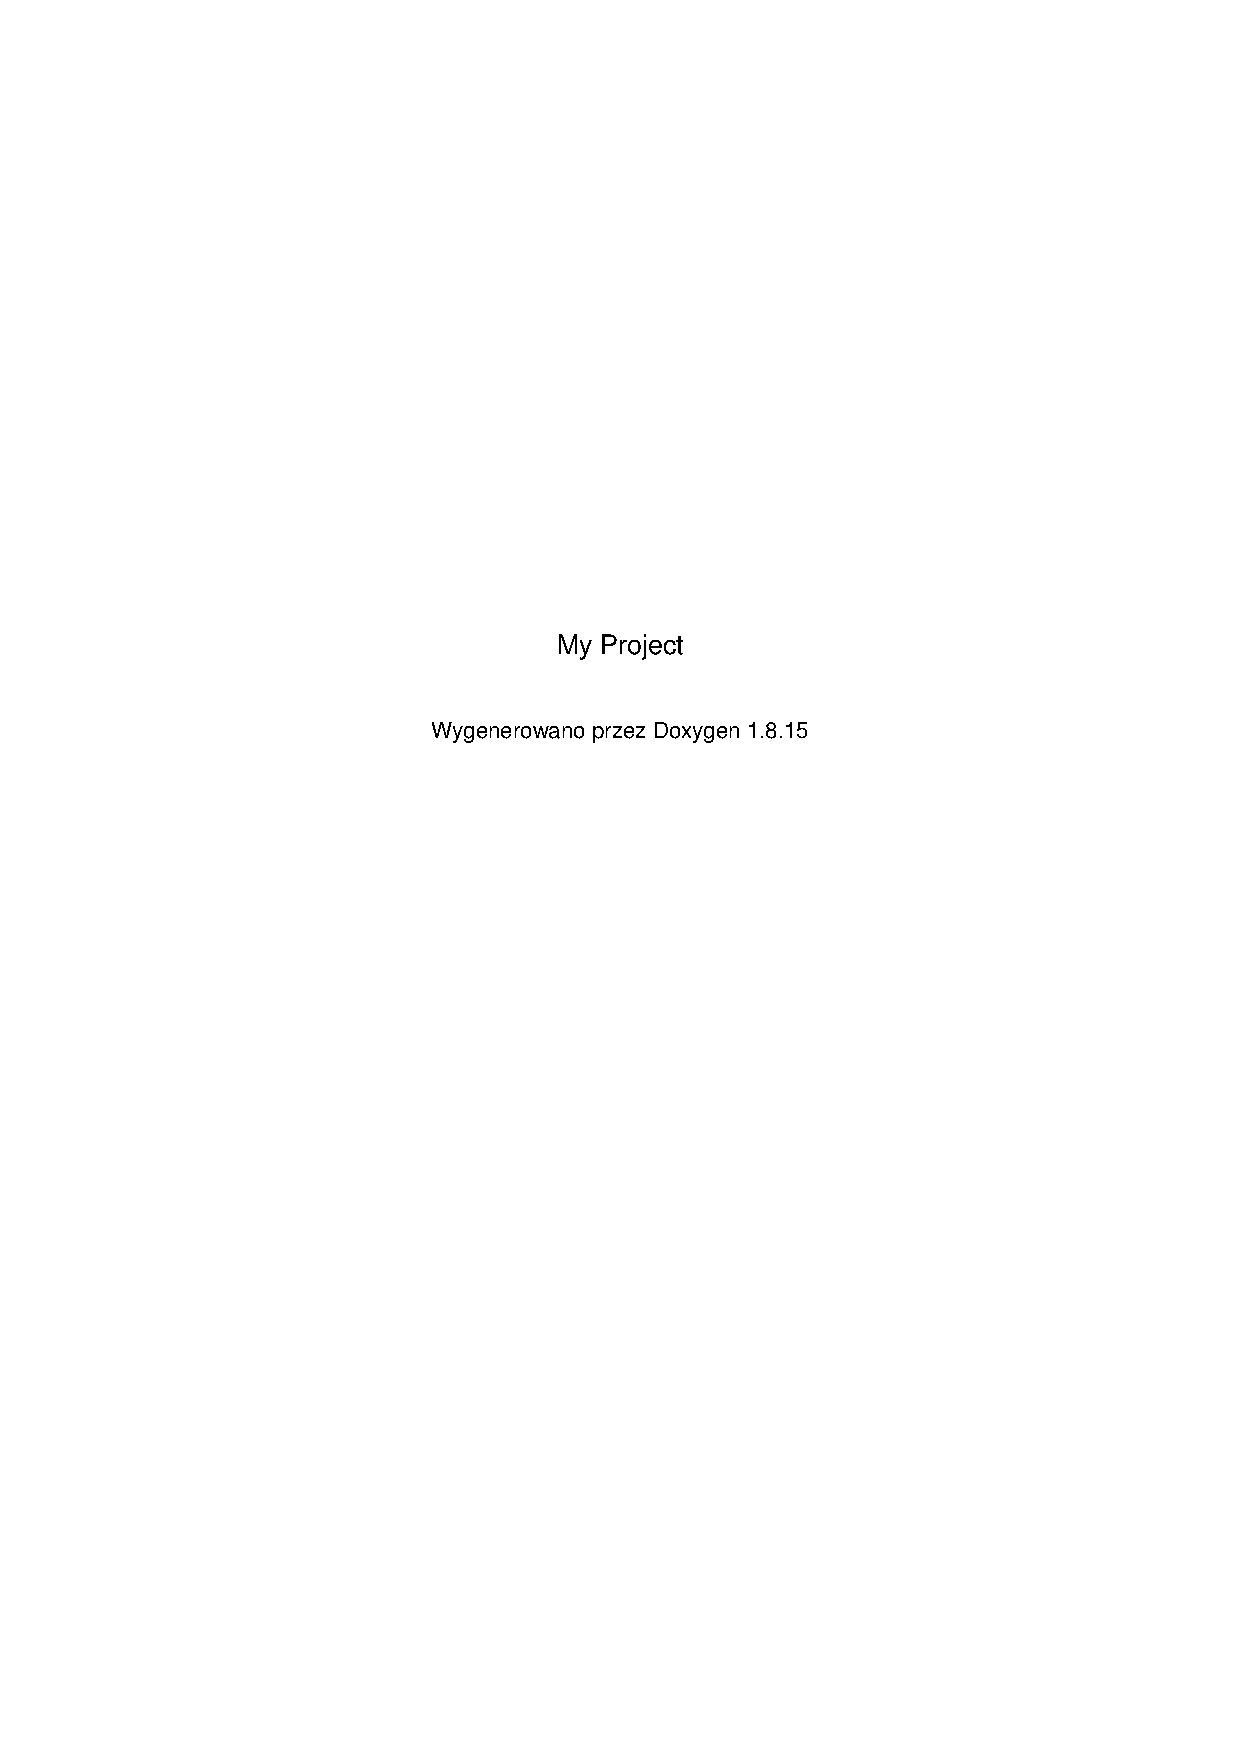
\includepdf[pages={1-36}]{refman.pdf}
\vfill 

\rule{0cm}{0cm}

\end{document}
% Koniec wieńczy dzieło.
